\section{Reflexive Modernization}

There is a transition from the `first modernity' to the `reflexive
modernity'. Society produces many (and new) side effects which can be
called `\textbf{manufactured risks}'.

These are unintended and cause uncertainty, but can be assessed, which
is `\textbf{reflexive introspection}'.

The old institutions cannot control these risks (they are
uncontrollable; see Risk Society), so they deny the risks; this is
`\textbf{organized irresponsibility}'. People are alienated from these
institutions because of this, and trust erodes.

\[
  \text{Modernization} \xrightarrow{\text{Creates}} \text{New risks}
  \xrightarrow{\text{Causes}} \text{Introspection of risks}
\]

Institutions losing out in the face of the reflexive modernity include:
\begin{itemize}
  \item The state loses power, non-state actors gain (corporations,
    NGOs etc).
  \marginpar{I assume that `womens liberation' (which appears in the
    lecture notes), is referring to a womans' ability to leave a
    family that doesn't work for her, or raise a family outside of the
    traditional `family construct'?}
  \item The family is splitting apart and divorce rates rise, womens
    liberation and work flexibility erode it.
  \item Religion loses power to secular institutions.
  \item Traditional political action fades as people don't identify
    strongly with a single party/ideology.
  \item Individualism rises.
\end{itemize}

\textbf{Example}
\begin{enumerate}
  \item Chernobyl blows up
  \item Increased critique about modern nuclear practice
  \item Widespread concern and distrust of industry, government and
    experts (established institutions)
  \item Increased regulation (to increase trust and decrease likelihood
    of another disaster)
  \item Slowed/abandoned expansion plans $\rightarrow$ modernity has
    altered course.
  \item \textbf{Reflexive modernization}.
\end{enumerate}

\section{Risk Society}

Modern society is increasingly structured around, and affected by new
qualities of risk that have not previously existed. The term was
coined by Ulrich Beck in 1986.

These risks are:
\begin{itemize}
  \item Invisible and undetectable except using science
  \item Universal; everybody is affected by them (even the rich, and
    those who produce the risk)
  \item Irreversible; we can't undo them
  \item The unknowns of the new risks are more important than the
    knowns. How can institutions manage this?
\end{itemize}

Environmental risk becomes the main product of modern society, and the
risks that we are exposed to are the product of the modernization
process itself.

\section{Planetary Boundaries and the Doughnut Economy}

Rockström proposed a framework of `planetary boundaries' which define
a safe space for humanity to develop within. If humanity stays within
these boundaries, then we are safe, but if we exceed any of the
boundaries, then we will be at risk of `irreversible and abrupt
environmental change'.

\begin{figure}[H]
 \centering
 \includesvg[width=0.5\columnwidth]{planetary-boundaries-2.svg}
 \caption{Planetary Boundaries}
\end{figure}

The Doughnut Economy is an economic model created by Kate Raworth which
focuses on everyone's right to basic needs such as food, education,
housing, etc, while not limiting opportunities for future generations
by protecting our ecosystem. This focus on well-being is at the expense
of economic growth.

\begin{figure}[H]
 \centering
 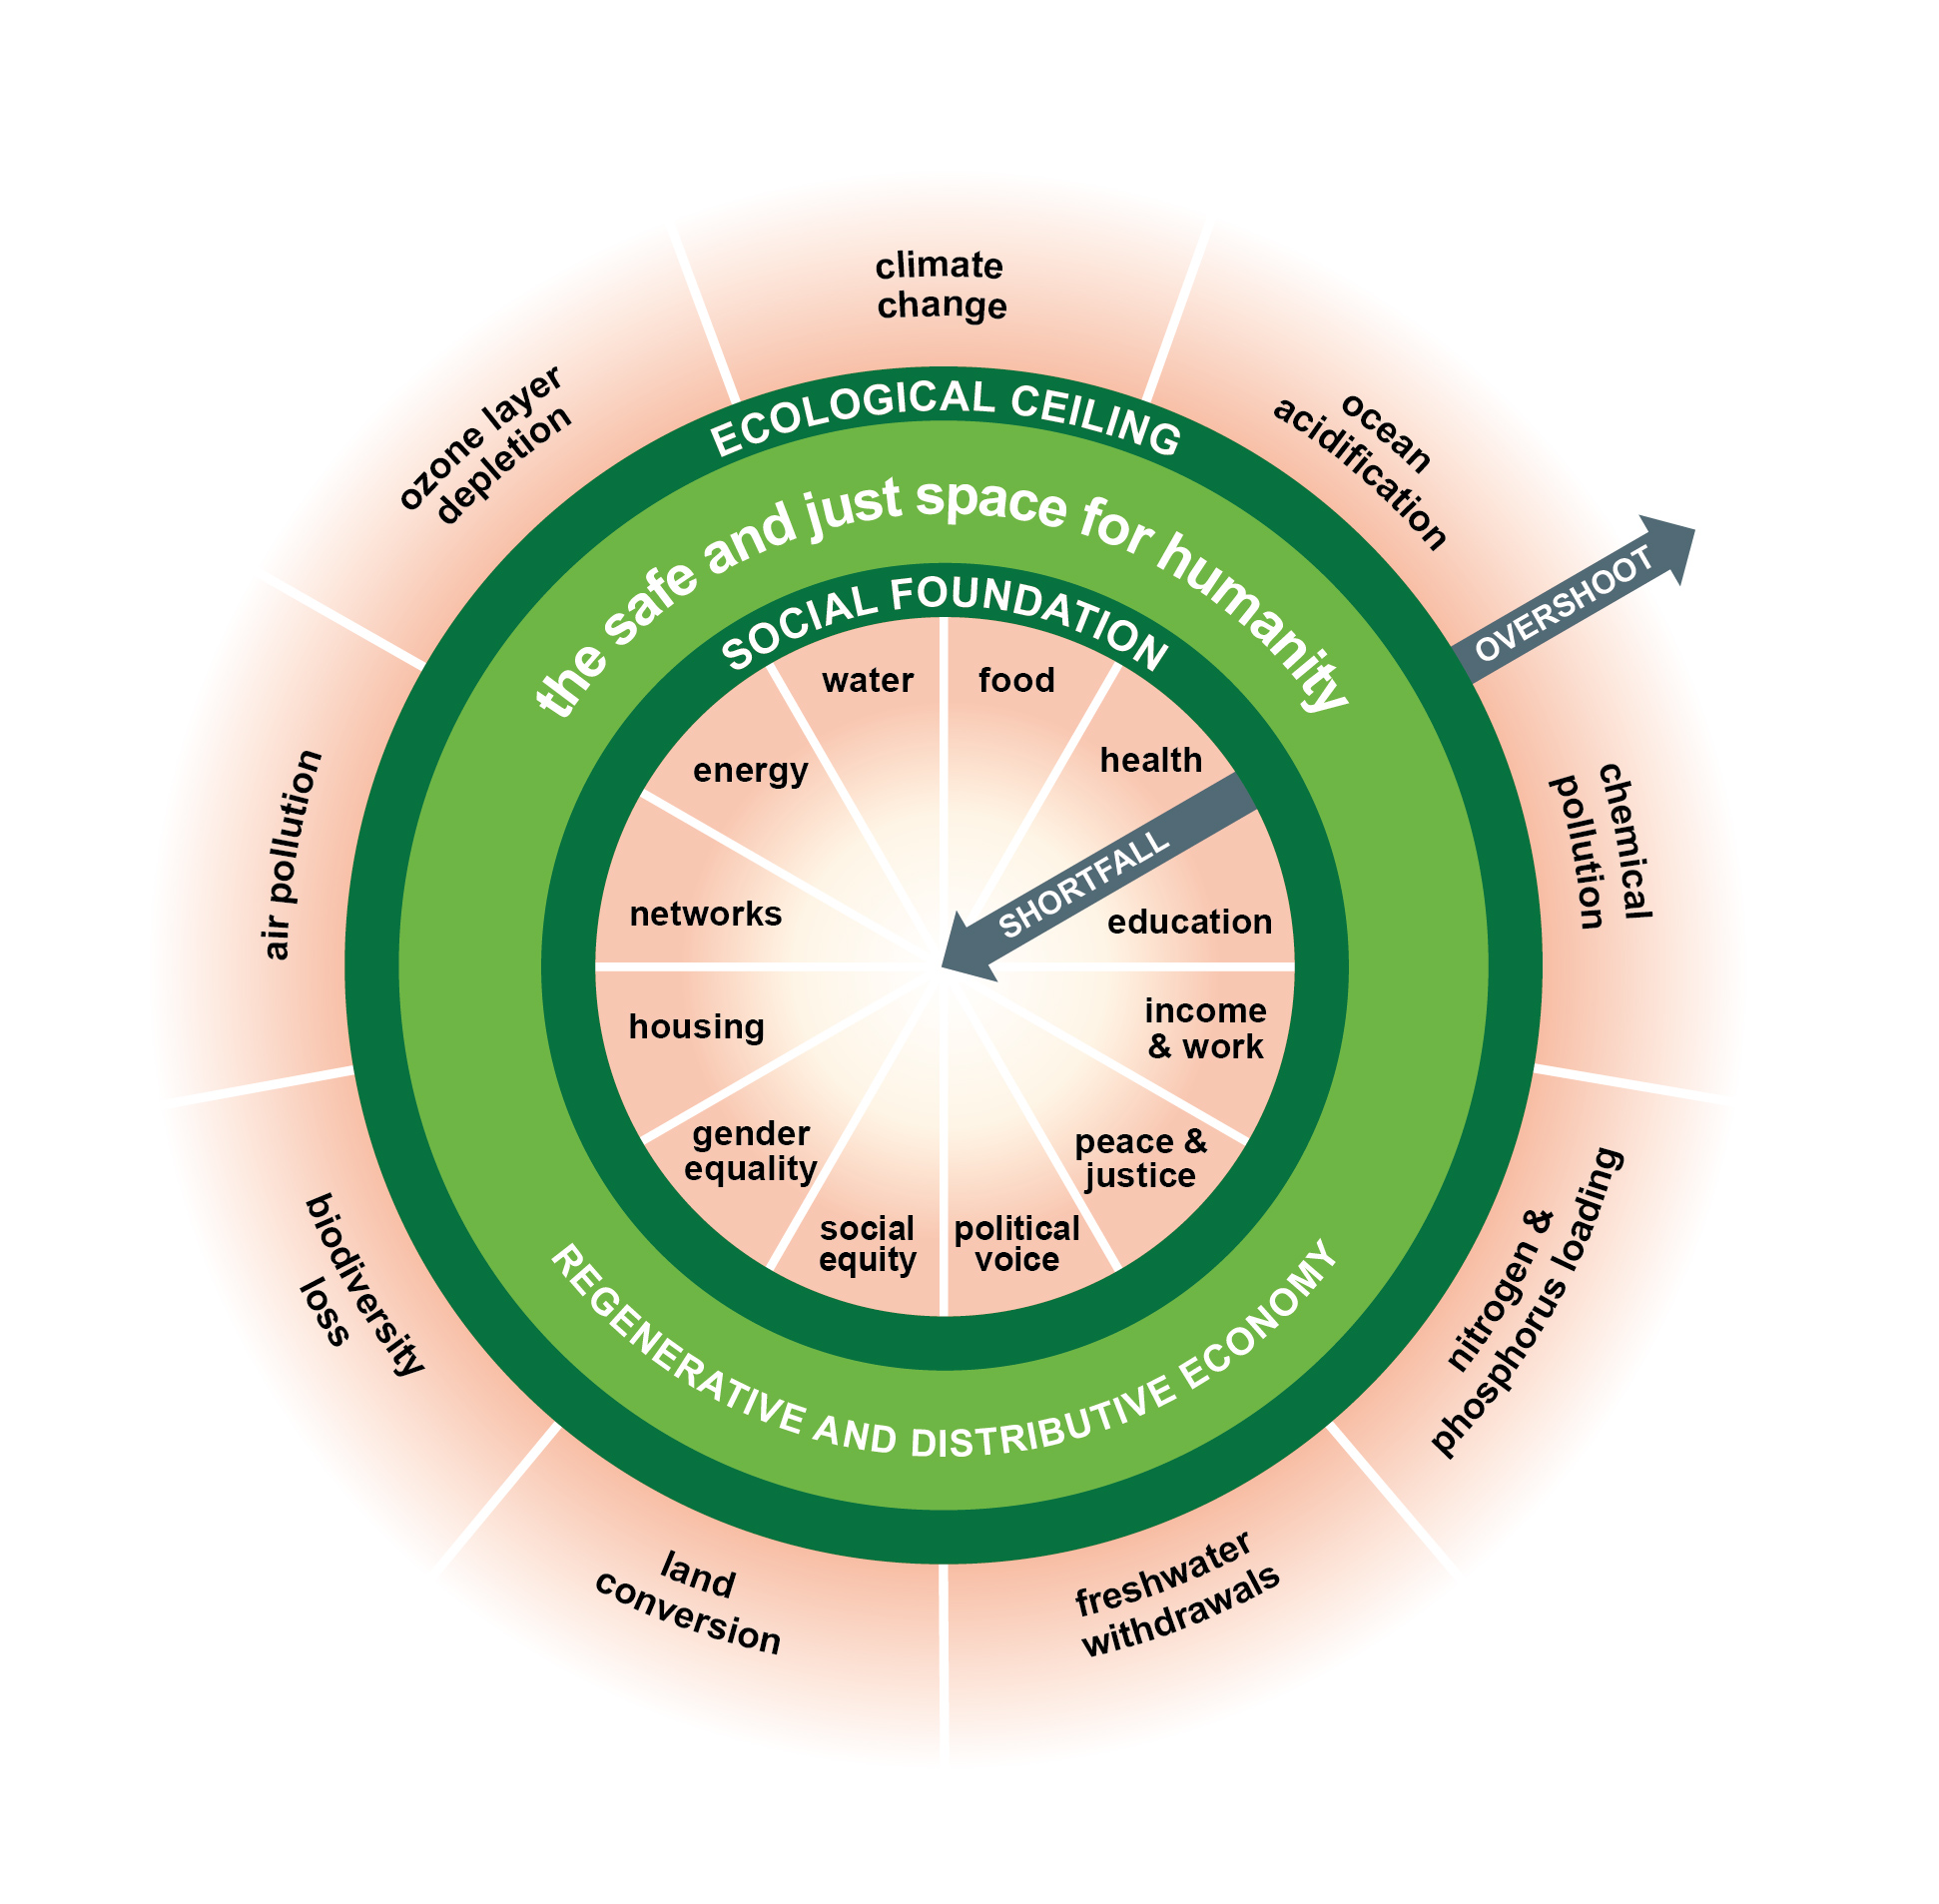
\includegraphics[width=0.6\columnwidth]{doughnut_economic_model.jpg}
 \caption{The Doughnut Economic Model}
\end{figure}

\section{Planning the Electricity Grid in Germany}

\textbf{Why does Germany need to expand the grid?}
\begin{itemize}
  \item There's lots more renewable energy generation which is
    volatile.
  \item The distance between energy production and consumption is
    increasing.
  \item Security of supply needs to continue (as the supply becomes
    more volatile and geographically distributed).
  \item Germany is a transit country for energy within the EU energy
    market.
  \item Grid expansion is cost effective for securing supply and
    competitive pricing; maximize utilization and ensure energy can
    always get to where it is needed. Transmission is currently a
    bottleneck for renewable expansion.
  \item Uncertainty of grid suitability for renewables makes renewable
    investment unattractive, which can jeopardize climate goals.
\end{itemize}

\textbf{How has the federal government responded?}
\begin{itemize}
  \item Created 5 laws/amendments to try to speed up grid procurement.
  \item Simplified the planning and approvals phases:
    \begin{itemize}
      \item Brought the whole process under the control of one federal
        ministry for streamlining.
      \item This ministry can see the bigger picture and is not as
        swayed by local concerns.
      \item Federal authorities apply the process with more
        consistency.
      \item Federal authorities have one set of rules, regulations and
        requirements.
      \item This process is now more transparent.
    \end{itemize}
  \item Increased incentives for expansion and optimization.
  \item Added regulations for financial compensation for landowners.
  \item Restricted the rights of federal states to oppose new grids,
    and put time limits on court challenges.
  \item Made less ugly underground cables the default over power
    lines, even though they're more expensive.
  \item Large energy consumers must have smart meters installed (even
    though the industry doesn't offer flexible tariffs yet, and it
    could be a cyber security risk).
\end{itemize}

\section{Nuclear Waste Siting}

\textbf{Technical Rationality} is a mind that puts faith in empirical
evidence and the scientific method. If emphasizes logical consistency
and universal impact.

\textbf{Cultural Rationality} gives weight to personal or familiar
experiences instead of depersonalized technical calculations, focusing
on the opinions of traditional and cultural norms, looking at
unanticipated consequences, and trusting process over outcome.

\textbf{Risk Assessment} emerged out of citizens not being able to
intelligently make decisions around technology and the environment. It
(broadly) doesn't work because the risks were assessed using technical
rationality, but they were interpreted through the lens of cultural
rationality.

People form a abstract knowledge structure called a `\textbf{schema}'
which they use to guide their perceptions and expectations. The schema
of a topic for a normal citizen is less refined than for an expert, so
when making decisions, citizens will fill the gaps with analogies and
experiences from their own lives.

Citizens often look closely at case-specific factors of an issue, and
examine the experts themselves. The latter point is important, since
often two experts can say different things based off of the same data,
forcing the citizens to choose who to trust. In situations where
deception is possible, or where there are high-stakes interests at
play, citizen scrutiny is highest because of this, which is rational.

The solution of Lasswell is that public debates should feature experts
who should interpret and present complex issues to the public to
facilitate citizen learning and empowerment, not just supply
information.

\section{Political Parties}

Political parties are central actors in democratic politics, and also
in many autocratic and totalitarian regimes. A `political party' has
no single definition, but generally means a group of people organizing
to win elections and control government.

Political parties
\begin{itemize}
  \item Coordinate between public officials, citizens with common
    (ideological or political) preferences and between citizens and
    officials.
  \item Define the agenda of elections.
  \item Select candidates to run in elections.
  \item Recruit for elections and for appointed office.
  \item Serve to represent the ideological positions and social
    groupings of citizens.
  \item Stabilize democracy by integrating new citizens (e.g. young
    people or immigrants) into the political system.
\end{itemize}

Problems parties face:
\begin{itemize}
  \item Increasing complexity, especially the pace of change and
    globalization.
  \item Increasing expectations of citizens towards individual
    politicians.
  \item Strike a balance between employing technocrats and experts to
    make decisions, and taking only a management role not a decision
    making or leadership role.
\end{itemize}

Also, how does society deal with successful anti-democratic parties?
Do they become integrated or socialized or do they undermine
democracy?

\section{Party Systems}

A party system is a set of parties that compete with the aim to
control government. The term only applies to democracies.

Political `cleavages' originate from socio-economic and cultural
divides. E.g. centralized areas vs regional areas, or secular
institutions vs religious institutions, or agrian parties vs pro
industrialization parties. Now we see a new environmental cleavage.

The rules of the electoral system are important for forming the
morphology (structure) of the party system. Party system types include
dominant party (one with many smaller parties), two party (e.g. the
UK), multi party (e.g. Germany) and bipolar (two large coalitions
which alternate).

`Centripetal party systems' concentrate power around the centre
(e.g. two party systems), and `centrifugal party systems' move power
towards the extremes. Plurality systems often produce two party
systems along the main cleavage (e.g. the UK) and proportional
representation systems often produce multiparty systems with many
interests (e.g. Germany).

In the `electoral market', the supply (parties) satisfy the demand
(voters) by positioning themselves as close to the political
preferences of as many voters as possible. They search for the sweet
spot where their support is largest. This is why parties move towards
the center in two-party systems; voters are least rigidly ideologized
there, and that's where the most votes are (most people are moderates).

\section{China's Governmental Structure}

\begin{itemize}
  \item In the past, lax enforcement of environmental legislation in
    China was blamed on local government. In a system of political
    competition, they would prioritize the main goal of economic
    growth over the sub-goal of environmental protection.
  \item Chinese leaders have been (re-)concentrating power back in the
    center, which could lead to improved environmental results.
  \item The behaviour of local officials has changed with increased
    attention and more financial resources.
  \item The strengthening of vertical linkage between the local
    government and the Ministry of Environment made falsifying
    information harder for local government, and thus harder to shirk
    policy implementation.
  \item There are still questions about the central government's
    commitment to better environmental governance, and even if it is
    fully motivated, it still needs good local information (which is
    improving, but as the Coronavirus outbreak shown, communication is
    not always smooth).
  \item There is no silver bullet, and recentralization certainly
    won't be one. Attention should be paid at all levels of the
    government hierarchy.
\end{itemize}

\section{Principle Agent Theory}

The principle-agent problem occurs when one entity (the agent) is able
to make decisions on behalf of another entity (the principle). A
dilemma occurs when agents are motivated to act in their own
interest, which is not aligned with that of the principle.

The special characteristics of the principle-agent relationship are:
\begin{enumerate}
  \item The relationship is asymmetric (the principle cannot know what
    the agent knows, or what the agent actually does).
  \item The principle depends on the agent.
  \item The principle must come up with strategies to remind the agent
    of its duties.
\end{enumerate}

\textbf{Shirking} is when the agent minimizes the effort it exerts on
behalf of the principle. \textbf{Slipping} is when the agent shifts
policy away from the principles towards outcome and towards its own
preferences.

\section{International Organizations}

An \textbf{International Organization} is a formal organization with a
permanent secretariat and at least three member states.

There have been many different `bigger picture' views on the purpose
of IOs over time.

\begin{description}
  \item[Functionalism] says that IOs serve a functional purpose, which
    is to minimize nationalism and territorial attachment in order to
    decrease conflict. The ultimate aim was to reduce the power of
    states and bring governments together through facilitating
    cooperation.
  \item[Neofunctionalism] was functionalism, with the additional goal
    that cooperation between states might spill over from one area to
    another, and cooperation would become increased, maybe eventually
    merging the states.
  \item[Hegemony Stability Theory] says that strong states (hegemons)
    were required to create regimes and IOs to facilitate their
    leadership. Hegemons create a `supply' of IOs and other states
    fulfill the demand. IOs serve to make the rule of the hegemons more
    efficient.

    Another view is that strong states would create IOs to voluntarily
    bind themselves and signal `strategic restraint' to reduce fear in
    smaller states. Either way, in HST, IOs serve the goals of
    hegemons.
  \item[Regime Theory] is where regimes (ran by IOs) are intervening
    variables between state preferences and outcomes. Regimes weren't
    really designed by states, but rather emerged as rules, norms,
    principles, etc that could shape state behaviour.
  \item[Keohane's Neoliberal Institutionalism] looks at the demand for
    IOs, and says that states create IOs when they have common
    interests in cooperation and the opportunity for mutual gains that
    they otherwise could not achieve.
  \item[Domestic benefits] can be derived through the joining of IOs,
    since it can signal to voters that a state is credible in its
    commitment to solving domestic problems that concern the IOs, and
    states benefit from the delegation of certain tasks to the IOs
    (e.g. monitoring and compliance verification).
\end{description}

Other IO fun facts that might come in handy:

\begin{description}
  \item[Rational Design] theory says that IOs are designed by states
    intentionally to solve problems.
  \item[Delegation Theory] uses Principle Agent theory to suggest that
    states are the principle and the IO is the agent. In theory, this
    reduces transaction costs and the IO is more efficient since it's
    specialized. In practice, the agent can shirk from its
    responsibilities.
  \item[IO Lifecycle] If the world changes, then the IO must be
    `recontracted', replaced or disbanded.
  \item[Preference Heterogeneity] is the extent to which individual
    tastes and preferences vary across actors. If the preference
    heterogeneity is high, then it means member states in an IO will
    find it harder to reach a consensus. It could then be harder to
    reform or recontract and IO.
  \item[Regionalism] notes that many IOs are regional and that a
    shared culture and aim helps create strong IOs.
    \begin{itemize}
      \item Shared external threats can create strong and `intrusive'
        IOs that closely coordinate states.
      \item Weak leaders who are worried about their own regime's
        survival aren't likely to secede sovereignty to an IO and thus
        give rise to less intrusive IOs.
    \end{itemize}
  \item[Legitimacy] is important for IOs since it makes them more able
    to sanction punitive action. Legitimacy can be derived in
    different ways, e.g. the UN Security Council is made up of 15
    members representing the heterogeneity of the international
    community.
  \item[Forum Shopping] is when actors look around for a `forum' to
    best achieve their goal in. For example, an actor could take its
    case to multiple criminal courts at once. This can cause IOs to
    have to compete, especially if they have overlapping concerns.
  \item[Emanations] are IOs created by other IOs. Often created by
    enterprising bureaucrats from the inside to make an entity not
    aligned with the views of the member states that make up the
    parent IO.
  \item[High Politics] refers to all matters relating to the very
    survival of a state (e.g. international security concerns).
  \item[Non-Governmental Organizations] often try to influence Key
    Opinion Formers in IOs and member states to change the status quo.
  \item[Bretton Woods Institutions] are the World Bank and the
    International Monetary Fund, which were founded in 1944 in Bretton
    Woods, US. Their aim was to re-build the shattered post WW2
    world-economy.
  \item[Rising Powers] are nations (or groups of nations) with an
    increasing primary influence in global affairs.
  \item[Multilateralism] is when an alliance of multiple countries
    pursue a common goal.
  \item[IOs are actors] in the sense that they have their own
    secretariat and staff, which have their own opinions. Though the
    IO is made up of and influenced by its members, its members itself
    are not able to fully influence the organisation.
  \item[Trust erosion] in IOs happens in three ways:
    \begin{itemize}
      \item Lack of transparency; events are unverifiable and happen
        behind closed doors.
      \item Exclusivity; affected citizens are not involved in
        decision making.
      \item Selectivity; problems are only tackled if they interest
        powerful actors.
    \end{itemize}
    IOs must therefore find ways to legitimize their decisions,
    respond to questions by civil society or states, and actively push
    against their own politicization to preserve their legitimacy.
\end{description}


\section{The EU}

The EU is complex, and made up of multiple parts; the European
Commission, the European Parliament, The European Court of Justice,
The European Council and The European Central Bank. The EU also has a
hierarchy of competence that it has control over, examples include:
\begin{description}
  \item[High/exclusive competence]- Customs union, monetary policy and
    competition law.
  \item[Shared competence] - Environmental policy, consumer protection
    and research.
  \item[Supporting competence] - Civil protection (e.g. police),
    education, culture.
\end{description}

The EU is able to be an actor in world politics due to:

\begin{description}
  \item[Presence] which is the ability of the EU to exert influence
    beyond its borders.
  \item[Opportunity] which is the external environment of ideas and
    events which constrain or enable 'actorness'.
  \item[Capability] is the internal context or view of the EU's
    external action; what does the EU think it is able to do?
  \item[Authority] is the legal competence of the EU in a given area.
  \item[Recognition] by other global actors, split into:
    \begin{description}
      \item[De jura recognition] which is diplomatic recognition in
        international law and formal membership in international
        organizations.
      \item[De factor recognition] which is recognition of an actor
        when third parties negotiate, who implicitly recognize it as an
        international actor.
    \end{description}
  \item[Internal cohesion] is the ability to formulate internally, and
    then represent an externally coherent position with a single
    voice, even if the agreed position is not the preferred position
    of each member state... and for individual member states to
    \textit{not} go behind the back of the EU in future negotiations.
\end{description}

\section{Brexit}

Brexit is the climax of UK skepticism of the EU. Citizens did not want
an `ever closer union', and recognized that the European Integration
process cannot be easily reversed. The challenge with the EU was to
speak with one voice during the negotiations, maintain internal
cohesiveness, and act effectively as an individual actor.

At the conception of the EU, the idea was that with the joint policy
projects in agriculture, the Euro, business, etc, beneficiaries would
be pro-integration as their lives intertwined with the EU. The EU was
originally promoted as a cognitive judgment and not linked to
emotional interests or nationalism. This is particularly relevant for
the UK and Denmark, who joined the EU on a mostly utilitarian and
transactional basis, which wasn't easily translated into a persuasive
narrative around cultural integration.

Accordingly, many of those now waiting European disintegration are
disadvantaged; there is a correlation between leave voters and
economic underdevelopment in the UK. Joining the EU in the first place
was the least-worst option for the British, never wanted a shared
European identity, didn't need the benefits of social rehabilitation
and reconstruction, and for who repeated exceptionalism (with respect
to EU legislation) became part of the political consciousness.

The paradox of the UK leaving the EU is that the UK heavily shaped the
EU, and Margret Thatcher (and the EU Commissioner from the UK at the
time) pushed heavily for the single market, common foreign and
security policy, and the integration of more Eastern European states.

Perhaps the EU needed more focus on its narrative from a sociological
standpoint at its inception, when it instead received lots of
political science and international relations analysis.

\section{Technology Assessment}

The motivation for TA is that technology produces solutions, but also
can cause unforeseen problems. The example is CRISPR which holds the
promise of treatments for disease that permeates many cells such as
cancer, aids or cystic fibrosis by editing DNA in live cells. The
concern is that CRISPR could have unexpected impacts once these
modified genes enter the gene pool.

We need TA because:
\begin{itemize}
  \item New technology creates problems in economic, political,
    technical, etc areas.
  \item \textit{Technology innovation expands but also restricts the
    capacity for action.}
  \item Open discussion between equals is a precondition for a
    constrictive debate on technology in society.
  \item History says that technology has risks, and expertocratic
    arrogance creates mistrust (see the Nuclear Waste Siting section).
  \item Decision making shouldn't be disconnected from those affected
    by the decisions.
\end{itemize}

\textbf{Technology Assessment} is ``A discipline of public
administration that seeks to build bridges between research and
innovation, society at large, and political decision process
makers.''. This allows an integration between the different kinds of
knowledge and different sets of values held by various social actors.

\textbf{Technology Evaluation} is the neutral and value-free
scientific recording of the consequences and side effects of
technology.

\textbf{Technology Impact Assessment} is a formal, evidence based
process that assesses the economic, social and environmental effects
of public policy and incorporates it into policy making. It is not
value-free, examining the impacts, the possible unintended
consequences and how the negative consequences could be mitigated.

\textbf{The Collingridge Dilemma} says that effects of a technology
cannot be easily predicted until the technology is sufficiently
developed and widely used, however, the more technology is widely
rooted in society, the harder it becomes to change it.

\textbf{The Precautionary Principle} says that even if there is an
incomplete knowledge of a topic or there is an absence of certainty,
we should attempt to avoid or minimize the potential for damage as far
as possible.

There are three `stages' that a technology can exist in; it starts as
`\textit{niche}' technology, then moves into a `\textit{transition}'
stage, before coming the `\textit{new system}'. Society needs a broad
range of technology in all stages: the niche stage creates space for
experimentation, the transition stage develops legal certainty and
promotes structural change, and the new system stage creates
stability.

\textbf{Constructive Technology Assessment} is based on the idea that
the future is predicated on the present, and the aim is to identify
emerging irreversabilities. ``\textbf{Enactors}'' try to realize new
technology and emphasize the positives, while ``\textbf{Comparative
  Selectors}'' develop ways to compare the enactors' options with
alternatives. Citizens and consumers can serve as amateur comparative
selectors.

TA is now embedded in lots of governmental structures, such as the EU,
the UK and the US.

The challenges around TA are mostly around it not being deeply
embedded in technology development, or not yet scaled up fully. There
needs to be more focus on societal well-being over economic growth,
more public and democratic discourse on science and technology
policy, more researchers and ethics committees that are connected to
decision markers, and more strategic, long term thinking.

\textbf{Research cultures} are the practices, norms and values that
characterize and guide knowledge production in a specific research
field. Science and technology policy needs a better understanding of
research cultures in order to direct research to create good and
societally beneficial research.

\section{Assorted definitions}

\subsection{The Rebound Effect}

The rebound effect (similar to the Jevons Paradox) is the reduction in
expected gains from an improvement efficiency on account of the
behavioral responses of actors using the technology that was
improved. Sometimes, the amount of a resource used can increase after
the improvement, which would be a `backfire' and is Jevons Paradox.

\subsection{Wicked Problem}

A Wicked Problem is a problem that is difficult or impossible to solve
because of incomplete, contradictory or changing requirements that are
often difficult to recognize.

\subsection{Policy Window}

A Policy Window is an unpredictable opening in the policy making
process which creates the possibility for an actor to influence the
direction and/or outcome of the process. Examples could be a cabinet
reshuffle, or a global event such as a pandemic.

\subsection{Constellation Analysis}

Constellation Analysis is a bridging concept for interdisciplinary and
transcisciplinary cooperation in various fields. It assumes that many
different factors (technical, social, natural) need to be considered
and related to each other.

The aim is to integrate different perspectives and approaches into one
model, analyze both general dynamics and specific situations and to
facilitate mutual understanding between different actors.

An \textbf{interdisciplinary approach} is solving problems using areas
of expertise from different disciplines.

A \textbf{transcisciplinary approach} is solving problems
collaboratively with both scientists and people from industry.

